%%%%%%%%%%%%%%%%%%%%%%%% Chapter 4: Method %%%%%%%%%%%%%%%%%%%%
%%%%%%%%%%%%%%%%%%%%%%%%%%%%%%%%%%%%%%%%%%%%%%%%%%%%%%%%%%%%%%%%%%%
%%%%%%%%%%%%%%%%%%%%%%%%%%%%%%%%%%%%%%%%%%%%%%%%%%%%%%%%%%%%%%%%%%%
%%%%%%%%%%%%%%%%%%%%%%%%%%%%%%%%%%%%%%%%%%%%%%%%%%%%%%%%%%%%%%%%%%%
\chapter{Proposed Methods}
\label{chapter:proposed_methods}
In Chapter 3, we explored clustering, vision transformers, and self-supervised learning frameworks like DINO and DINOv2, including their evaluation in various scenarios. Building on that, Chapter 4 outlines our proposed methods and the steps involved in our experiments. We start with how we created our image datasets using annotation files provided for DAA video dataset, including addressing dataset imbalance and relevant statistics. We introduce a new dataloader designed specifically for imbalanced datasets and describe our clustering process. The chapter also explains our methodologies for comparing new dataloader with traditional one and training and evaluating our models. Additionally, we provide necessary mathematical formulations to aid in understanding our evaluation principles, and we outline our experimental goals, which will be tested in the following chapter.

\section{Image Dataset Generation}
This section explains how we created image datasets from the \gls{daa} video dataset~\citep{martin2019drive_and_act_2019_iccv} using the provided annotation files. First, we'll examine the structure of these annotation files to understand how to extract frames from the \gls{daa} videos. We'll then go over the data pre-processing steps and frame extraction process. By the end of this section, we'll have prepared the extracted image datasets for an analysis of any imbalances in the next section.

\paragraph{Dataset Annotation Details:} The annotation files are integral for indexing and extracting relevant frames. An example of such a file,~``midlevel.chunks\_90.split\_0.train.csv", provided by \gls{daa}~\citep{martin2019drive_and_act_2019_iccv} video dataset, is depicted in the figure~\ref{fig:example of an annotation file}. It includes headers like participant\_id, file\_id, annotation\_id, frame\_start, frame\_end, activity, and chunk\_id. For instance, entries in this file indicate specific activities such as `closing\_door\_outside' and `opening\_door\_outside', with precise frame ranges provided for effective localization of the activity within the video because each activity is captured for 3 seconds and corresponds to 1 video sample~\citep{martin2019drive_and_act_2019_iccv}.

\begin{figure}[h]
\begin{center}
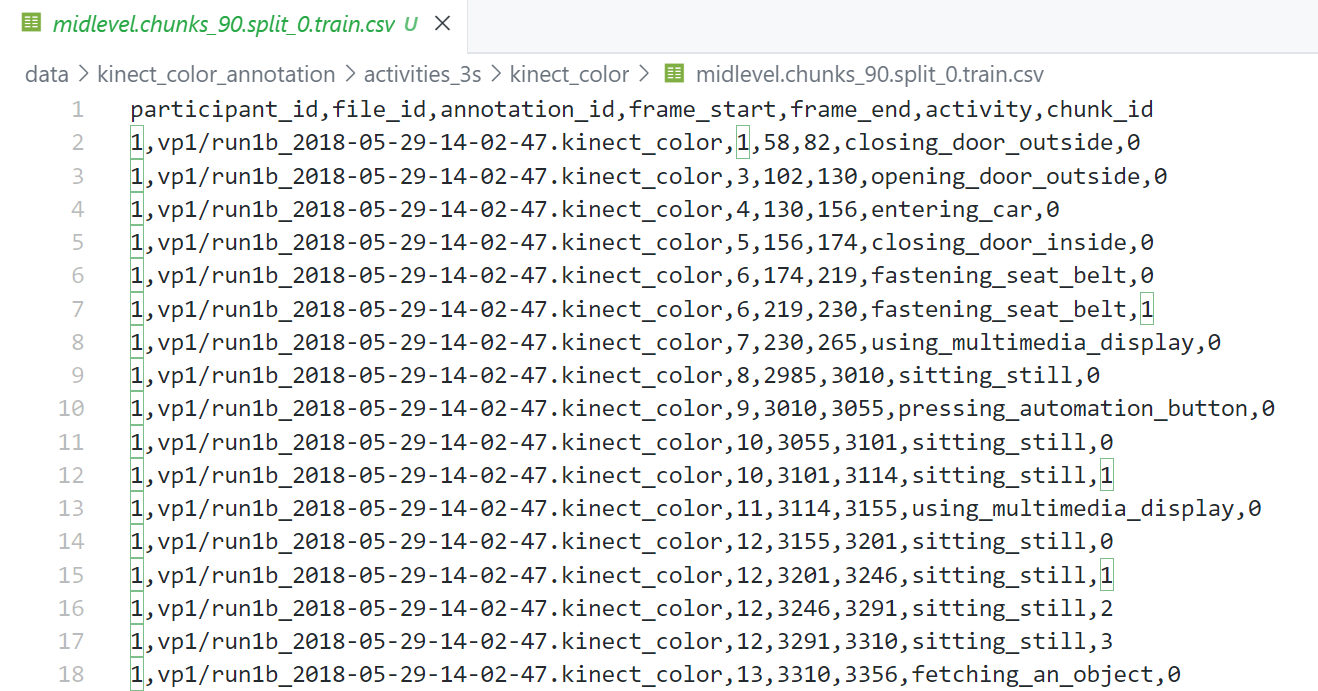
\includegraphics[width=0.8\textwidth]{Images_Thesis/annotation_example.png}
\end{center}
\caption[Example of an annotations file.]{This figure depicts the annotation structure in the ``midlevel.chunks\_90.split\_0.train.csv" file provided by~\citet{martin2019drive_and_act_2019_iccv} for the train dataset of the split 0 of the Kinect Color \gls{daa} video dataset.It includes headers like participant\_id, file\_id, annotation\_id, frame\_start, frame\_end, activity, and chunk\_id. These details are utilized to extract exact image frames corresponding to each activity in the \gls{daa} video dataset.}
\label{fig:example of an annotation file}
\end{figure}

\paragraph{Data Preprocessing and Frame Extraction:} The methodology's initial step involves extracting image frames from the video files of the \gls{daa} dataset. This process forms foundational image datasets corresponding to each considered modality and camera view. Table~\ref{table for views and modalities in daa dataset} contains information about different modalities and views offered by \gls{daa} dataset~\citet{martin2019drive_and_act_2019_iccv}. Specifically, two camera views are utilized for this research: the `Right Top View' and the `Front Top View' as depicted in the table~\ref{table for views and modalities used in this thesis}. Two `Right Top View' datasets come from color and infrared videos captured by the Kinect camera and one `Front-top View' dataset comes from NIR camera recordings. Table~\ref{table for different daa dataset versions formed in this thesis} lists the different image datasets obtained as a results of frame extraction procedure on the \gls{daa} video dataset. Additionally, it includes details regarding the specific perspective captured in the dataset, as well as the designated name for the image dataset within the context of this thesis. The number of channels in the table~\ref{table for different daa dataset versions formed in this thesis} includes information about the number of channels in each image, where for gray scale images there are 3 channels in which each channel contains the same information or in other words one gray scale channel is repeated thrice. This thesis focuses on training models using the `Kinect Right Top View' color \gls{daa} dataset and evaluating their performance on Infrared (Grayscale) datasets to assess their ability to generalize across different modalities and viewpoints.

\paragraph{Dataset Categorization:} This thesis focuses on driver distraction, which necessitates a streamlined approach to data categorization. The extracted drive and act image datasets, consisting of 34 distinct midlevel activities that detail various driver behaviors, are further reorganised into two main classes: `\_non\_distracted' and `distracted' driver. The `\_non\_distracted' class includes activities that indicate the driver's full attention to driving. For example, the `sitting\_still' activity is clearly aligned with a non-distracted state. Similarly, activities like `entering\_car' and `exiting\_car', which occur outside the active driving period, are also grouped under `non\_distracted'. Alternatively, these activities could be excluded altogether, allowing the analysis to focus strictly on a binary classification: `sitting\_still' versus all other activities. 

In contrast, the `distracted' class comprises the remaining 31 fine-grained activities depicted in figure~\ref{fig:driveandact_activities}, representing potential distractions from the driving task. This binary categorization simplifies the dataset, enhancing its compatibility with the PyTorch Image Folder class~\citep{torchvision_imagefolder}.

\begin{table}[t]
\caption[Different views and modalities in Drive and Act Dataset.]{Different views and modalities in Drive and Act Dataset. Source:~\citep{martin2019drive_and_act_2019_iccv}}
\label{table for views and modalities in daa dataset}
\begin{center}
\small
\begin{tabular}{lll}
\multicolumn{1}{c}{\bf Camera Type}  &\multicolumn{1}{c}{\bf Modality Type} &\multicolumn{1}{c}{\bf View Type}
\\ \hline 
NIR         & Infra-red (Gray scale)  &Front Top
\\ \hline
NIR         & Infra-red (Gray scale)  &Right Top
\\ \hline 
NIR         & Infra-red (Gray scale)  &Back
\\ \hline 
NIR         & Infra-red (Gray scale)  &Face view
\\ \hline 
NIR         & Infra-red (Gray scale)  &Left Top
\\ \hline 
Kinect         & Color (RGB)  &Right Top
\\ \hline 
Kinect         & Depth  &Right Top
\\ \hline 
Kinect        & Infra-red (Gray scale)  &Right Top
\\ \hline 
\end{tabular}
\end{center}
\end{table}

\begin{table}[t]
\caption[Different views and modalities from Drive and Act Dataset used in this thesis.]{Different views and modalities from Drive and Act Dataset used in this thesis. Source:~\citep{martin2019drive_and_act_2019_iccv}}
\label{table for views and modalities used in this thesis}
\begin{center}
\small
\begin{tabular}{lll}
\multicolumn{1}{c}{\bf Camera Type}  &\multicolumn{1}{c}{\bf Modality Type} &\multicolumn{1}{c}{\bf View Type}
\\ \hline 
NIR         & Infra-red (Gray scale)  &Front Top
\\ \hline 
Kinect         & Color (RGB)  &Right Top
\\ \hline 
Kinect        & Infra-red (Gray scale)  &Right Top
\\ \hline
\end{tabular}
\end{center}
\end{table}

\begin{table}[t]
\caption[Different version of Drive and Act (DAA) Image Datasets formed in this thesis.]{Different version of Drive and Act (DAA) Image Datasets formed in this thesis. Source:~\citep{martin2019drive_and_act_2019_iccv}}
\label{table for different daa dataset versions formed in this thesis}
\begin{center}
\small
\begin{tabular}{llll}
\multicolumn{1}{c}{\bf Camera and Modality Type}  &\multicolumn{1}{c}{\bf View Type} &\multicolumn{1}{c}{\bf Dataset Name} &\multicolumn{1}{c}{\bf Number of Channels}
\\ \hline 
Near Infra-red (Gray scale)  &Front Top & NIR Front Top Image DAA & 1 x 3 (duplicated)
\\ \hline 
Kinect Color (RGB)  &Right Top & Kinect Color Right Top Image DAA & 3 (RGB)
\\ \hline 
Kinect Infra-red (Gray scale)  &Right Top & Kinect IR Right Top Image DAA & 1 x 3 (duplicated)
\\ \hline
\end{tabular}
\end{center}
\end{table}

\subsection{Dataset Statistics}
\label{section:Imbalance and Dataset Statistics}
After extracting the image datasets into 34 fine grained activities, there is evidence of significant disparities in class distribution within the resulted image datasets.~Figure~\ref{fig:driveandact_multi_class_imbalance_split_0} illustrates the disparities among the 34 fine-grained activities in `split 0' of the `Kincet Color Right Top Image DAA' train dataset. The dataset for this split contains a total of 259,865 images. Of these, the `sitting\_still' class alone comprises 78,227 images, which account for 30.10\% of the dataset. This starkly contrasts with categories such as `closing\_door\_outside,' which represents a mere 0.087\% with only 226 images. Such imbalances highlight the challenges in training models that can accurately recognize less frequent activities. However, this view gives us multi-class classification perspective of the image datasets and we need to further analyse the statistics for the binary classification task `non distracted' driver versus `distracted' driver. The imbalance ratio~\citep{23_ImR_buda2018systematic} is used as a standard metric to calculate the imbalance with respect to minority and majority classes rather than class ratios with respect to whole dataset size.
%%%%%%%%%%%%%%%%%%%%%%%%%%%%%%%%%%%%%%%%%%%%%%%%%%%%%%%%%%%%%%%%
%%%%%%%%%%% Class ratios figure split_0 Color DAA %%%%%%%%%%%%
\begin{figure}[h]
\begin{center}
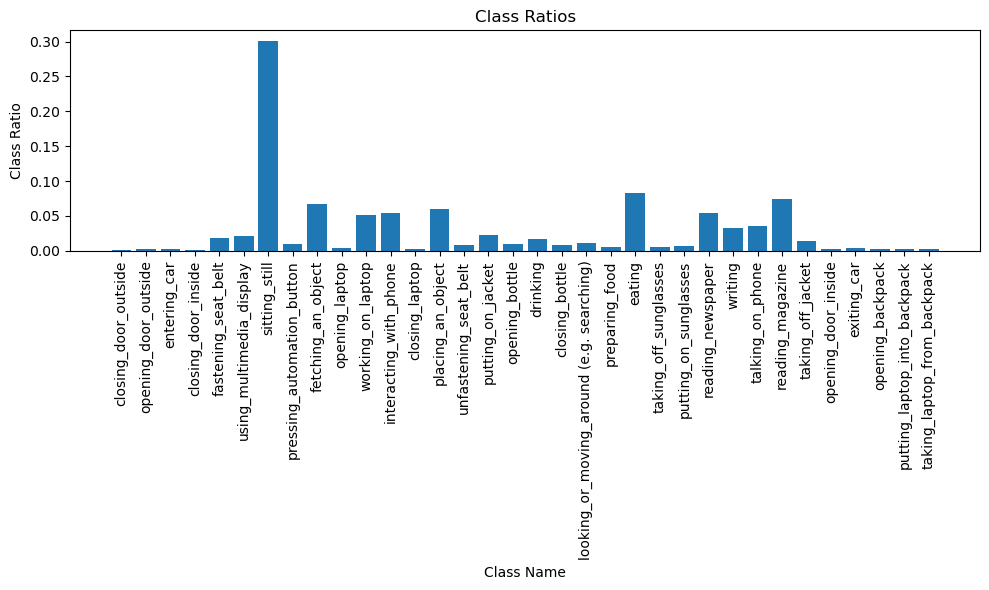
\includegraphics[width=0.8\textwidth]{Images_Thesis/daa_images/class_ratios_spli_0_train_output.png}
\end{center}
\caption[Illustrative image depicting the class imbalance in the split 0 of the Kincet Color Right Top Image DAA train dataset with 34 fine grained activities.]{Illustrative image depicting the class imbalance in the split 0 of the Kincet Color right Top Image DAA train dataset with 34 fine grained activities. The y-axis represents the class ratios and the x-axis represents 34 fine-grained activities. This extracted image dataset can be used for multi-class classification tasks like driver action recognition.}
\label{fig:driveandact_multi_class_imbalance_split_0}
\end{figure}

\paragraph{Method to calculate the class ratios}
Suppose we have a dataset with 34 distinct classes. Let \( N \) be the total number of images in the train set of split 0 of the `Kinect Color Right Top \gls{daa}' dataset, and let \( N_i \) be the number of images in each class \( C_i \) for \( i = 1, 2, \ldots, 34 \).

The class ratio \( R_i \) for each class \( C_i \) with respect to the total dataset is defined as:
\begin{equation}
\begin{aligned}
R_i = \frac{N_i}{N}
\end{aligned}
\label{equation:4.1}
\end{equation}
which gives the proportion of elements in each class relative to the entire dataset~\citep{Survey_DL_Taghi_article, 23_ImR_buda2018systematic}.

To convert this class ratio into a proportional percentage, which expresses the proportion of each class as a percentage of the total dataset, we multiply the class ratio by 100~\citep{book_stat_ratios_bennett2003statistical}. Thus, the proportional percentage \( P_i \) is defined as:
\begin{equation}
\begin{aligned}
P_i = R_i \times 100
\end{aligned}
\label{equation:4.2}
\end{equation}
This provides the percentage of the dataset that belongs to each class, facilitating easier comparison and visualization of class distribution.

Furthermore, for any two different classes \( C_i \) and \( C_j \) with \( N_i \) and \( N_j \) denoting the number of elements in each class , the pairwise class ratio \( R_{ij} \) can be defined as:
\begin{equation}
\begin{aligned}
R_{ij} = \frac{N_i}{N_j}
\end{aligned}
\label{equation:4.3}
\end{equation}
which compares the relative sizes of any two classes.

For example, the class ratio for `sitting\_still' class can be calculated as follows:
\[
R_i = \frac{78227}{259865} = 0.3010
\]
And, the proportional percentage for `sitting\_still' class can be calculated as follows:
\[
P_i = 0.3010 \times 100 = 30.10\%
\]

\subsection{Imbalance Across Different Splits and Classes}

The datasets further contains the imbalance between `\_non-distracted' and `distracted' driver classes across each dataset split. Figure~\ref{fig:Class_dist_whole_grid_Kinect_color} shows the distribution of `\_non-distracted' and `distracted' driver classes in the Kinect color Right Top Image DAA Dataset. Tables~\ref{kir imbalance-table} to~\ref{nir imbalance-table}, presents the imbalance ratio (ImR) for all generated image datasets. The Imbalance Ratio (ImR) is the ratio of image count for the majority class (`distracted') to the image count for the minority class (`non-distracted')~\citep{Survey_DL_Taghi_article, 23_ImR_buda2018systematic}. This metric shows the significant skew in data distribution, affecting the training and performance of detection models.

For a binary classification dataset, mathematically, the Imbalance Ratio can be written as follows:
\begin{equation}
\begin{aligned}
ImR = \frac{N_{Majority}}{N_{Minority}}
\end{aligned}
\label{equation:4.4}
\end{equation}
where \(N_{Majority}\) represents the total number of images in the majority class and \(N_{Minority}\) represents the total number of images in the minority class~\citep{Survey_DL_Taghi_article, 23_ImR_buda2018systematic}.

%%%%%%%%%%%%%%%%%%%%%%%%%%%%%%%%%%%%%%%%%%%%%%%%%%%%%%%%%%%%%%%%
%%%%%%%%%%% Tables for Imabalnced Ratio %%%%%%%%%%%%
\begin{table}[htbp]
\caption{Imbalance in Kinect Color Right Top Image DAA Dataset}
\label{rgb imbalance-table}
\begin{center}
\small
\begin{tabular}{llllll}
\multicolumn{1}{c}{\bf Dataset Split}  &\multicolumn{1}{c}{\bf Modality} &\multicolumn{1}{c}{\bf View} &\multicolumn{1}{c}{\bf ImR Train} &\multicolumn{1}{c}{\bf ImR Validation} &\multicolumn{1}{c}{\bf ImR Test}
\\ \hline \\
Split\_0         &Kinect RGB  &Right Top  &$\frac{179931}{79934} = 2.25$ & $\frac{43703}{12321} = 3.54$ & $\frac{55930}{31385} = 1.78$  \\
\\ \hline \\
Split\_1             &Kinect RGB  &Right Top  &$\frac{190562}{94245} = 2.02$ & $\frac{37934}{16607} = 2.28$ & $\frac{51068}{12788} = 3.99$ \\
\\ \hline \\
Split\_2             &Kinect RGB & Right Top & $\frac{188635}{73101} = 2.58$ & $\frac{34274}{19638} = 1.74$ & $\frac{56655}{30901} = 1.83$\\
\\ \hline
\end{tabular}
\end{center}
\end{table}

%%%%%%%%%%%%%%%%%%%%%%%%%%%%%%%%%%%%%%%%%%%%%%%%%%%%%%%%%%%%%%%%%
\begin{table}[htbp]
\caption{Imbalance in Kinect IR Right Top Image DAA Dataset}
\label{kir imbalance-table}
\begin{center}
\small
\begin{tabular}{llllll}
\multicolumn{1}{c}{\bf Dataset Split}  &\multicolumn{1}{c}{\bf Modality} &\multicolumn{1}{c}{\bf View} &\multicolumn{1}{c}{\bf ImR Train} &\multicolumn{1}{c}{\bf ImR Validation} &\multicolumn{1}{c}{\bf ImR Test}
\\ \hline \\
Split\_0         &Kinect Infra Red  &Right Top  & $\frac{209827}{87758} = 2.39$ & $\frac{50465}{13721} = 3.67$ & $\frac{64799}{34347} = 1.88$ \\
\\ \hline \\
Split\_1             &Kinect Infra Red  &Right Top  & $\frac{221575}{103027} = 2.15$ & $\frac{44258}{18448} = 2.399$ & $\frac{59258}{14351} = 4.129$ \\
\\ \hline \\
Split\_2             &Kinect Infra Red & Right Top & $\frac{218780}{80867} = 2.70$ & $\frac{40313}{21490} = 1.87$ & $\frac{65998}{33469} = 1.97$  \\
\\ \hline
\end{tabular}
\end{center}
\end{table}

%%%%%%%%%%%%%%%%%%%%%%%%%%%%%%%%%%%%%%%%%%%%%%%%%%%%%%%%%%%%%%%
\begin{table}[htbp]
\caption{Imbalance in Near Infra Red Front Top Image DAA Dataset}
\label{nir imbalance-table}
\begin{center}
\small
\begin{tabular}{llllll}
\multicolumn{1}{c}{\bf Dataset Split}  &\multicolumn{1}{c}{\bf Modality} &\multicolumn{1}{c}{\bf View} &\multicolumn{1}{c}{\bf ImR Train} &\multicolumn{1}{c}{\bf ImR Validation} &\multicolumn{1}{c}{\bf ImR Test}
\\ \hline \\
Split\_0         &Near Infra Red  &Front Top  & $\frac{351345}{156522} = 2.24$ & $\frac{85400}{24101} = 3.54$ & $\frac{109493}{61492} = 1.78$ \\
\\ \hline \\
Split\_1             &Near Infra Red  &Front Top & $\frac{371987}{184436} = 2.01$ & $\frac{74304}{32598} = 2.27$ & $\frac{99947}{25081} = 3.98$ \\
\\ \hline \\
Split\_2             &Near Infra Red & Front Top & $\frac{369144}{143272} = 2.57$ & $\frac{67123}{38541} = 1.74$ & $\frac{109971}{60302} = 1.82$  \\
\\ \hline
\end{tabular}
\end{center}
\end{table}

%%%%%%%%%%%%%%%%%% Grid of class distributions %%%%%%%%%%%%%%%%%
\begin{figure}[htbp]
    \centering
    % First row
    \begin{subfigure}[b]{0.45\textwidth}
        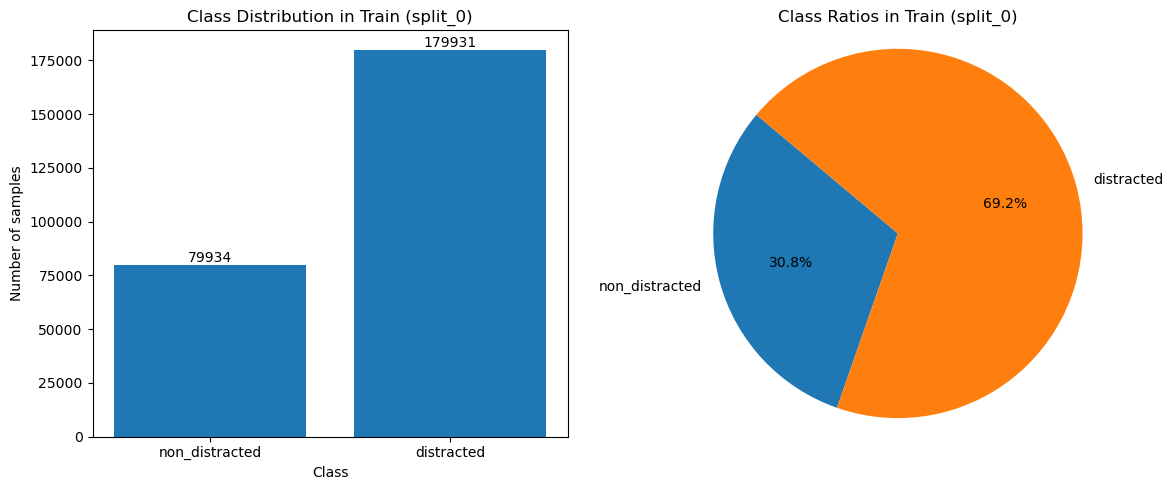
\includegraphics[width=\textwidth]{Images_Thesis/class_distribution_Kinect_color/split_0_rgb_daa/class_dist_train_sp_0_rgb_daa.png}
        \caption{Split 0: Train}
        \label{fig:Class_dist_grid_image1}
    \end{subfigure}
    \hfill % space between images
    \begin{subfigure}[b]{0.45\textwidth}
        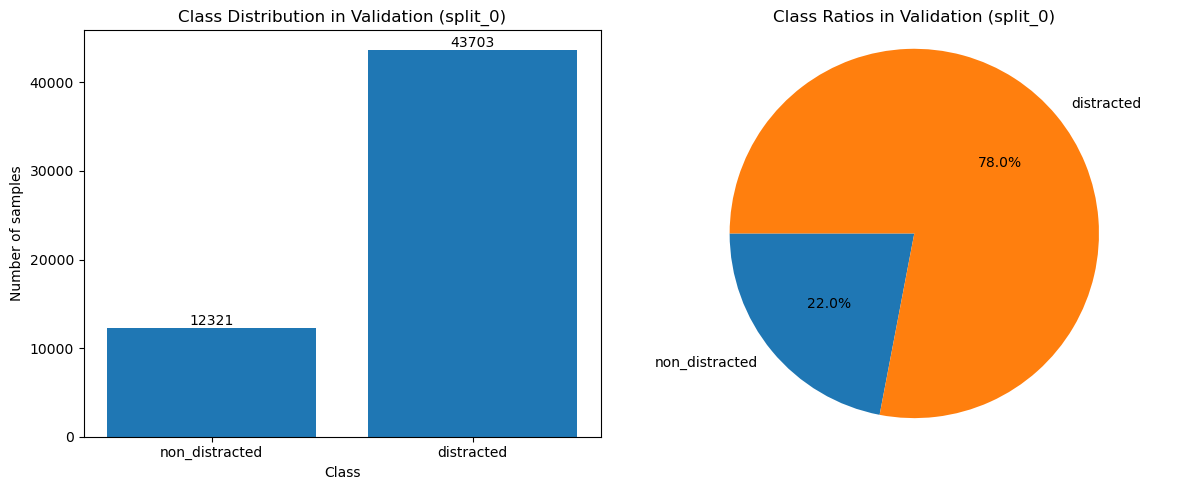
\includegraphics[width=\textwidth]{Images_Thesis/class_distribution_Kinect_color/split_0_rgb_daa/class_dist_val_sp_0_rgb_daa.png}
        \caption{Split 0: Validation}
        \label{fig:Class_dist_grid_image2}
    \end{subfigure}

    % Second row
    \begin{subfigure}[b]{0.45\textwidth}
        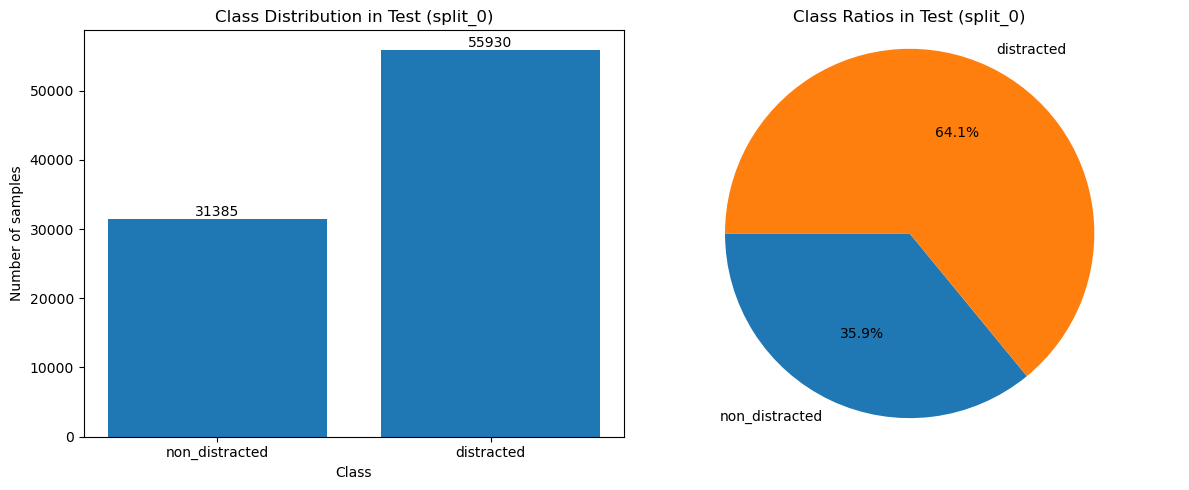
\includegraphics[width=\textwidth]{Images_Thesis/class_distribution_Kinect_color/split_0_rgb_daa/class_dist_test_sp_0_rgb_daa.png}
        \caption{Split 0: Test}
        \label{fig:Class_dist_grid_image3}
    \end{subfigure}
    \hfill
    \begin{subfigure}[b]{0.45\textwidth}
        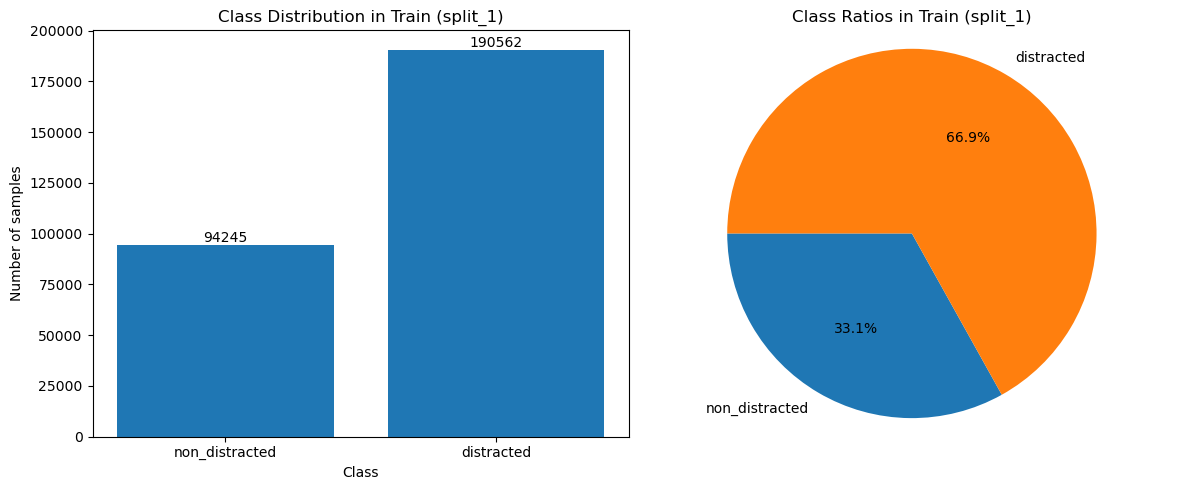
\includegraphics[width=\textwidth]{Images_Thesis/class_distribution_Kinect_color/split_1_rgb_daa/class_dist_train_rgb_sp_1_daa.png}
        \caption{Split 1: Train}
        \label{fig:Class_dist_grid_image4}
    \end{subfigure}

    % Third row
    \begin{subfigure}[b]{0.45\textwidth}
        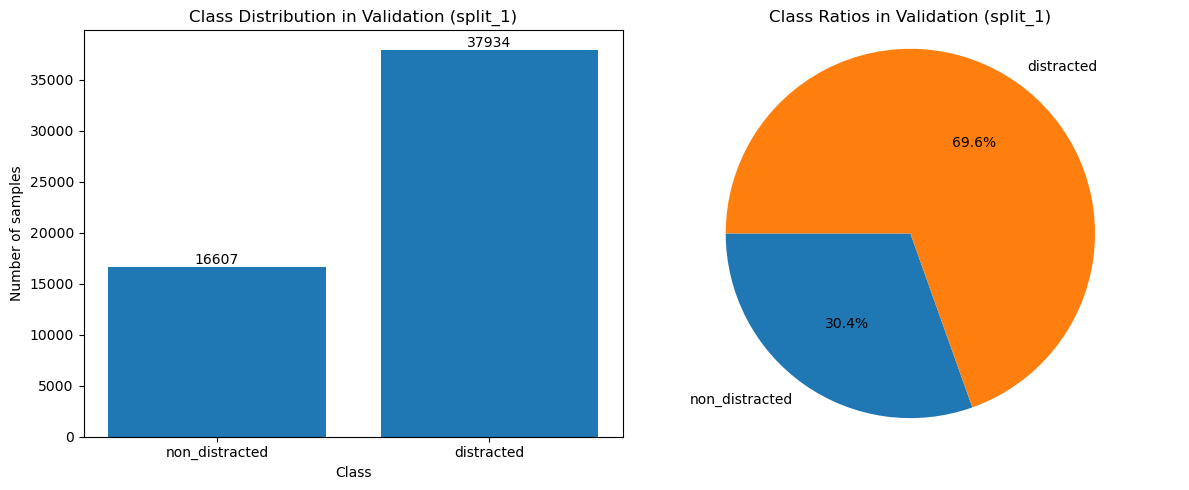
\includegraphics[width=\textwidth]{Images_Thesis/class_distribution_Kinect_color/split_1_rgb_daa/class_dist_val_sp_1_rgb_daa.png}
        \caption{Split 1: Validation}
        \label{fig:Class_dist_grid_image5}
    \end{subfigure}
    \hfill
    \begin{subfigure}[b]{0.45\textwidth}
        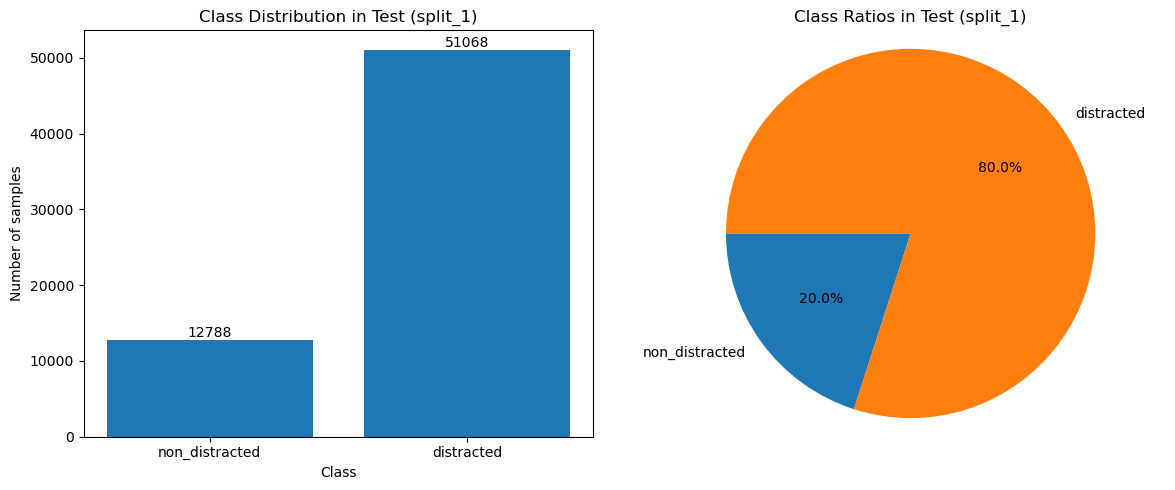
\includegraphics[width=\textwidth]{Images_Thesis/class_distribution_Kinect_color/split_1_rgb_daa/class_dist_test_sp_1_rgb_daa.png}
        \caption{Split 1: Test}
        \label{fig:Class_dist_grid_image6}
    \end{subfigure}

    % Fourth row
    \begin{subfigure}[b]{0.45\textwidth}
        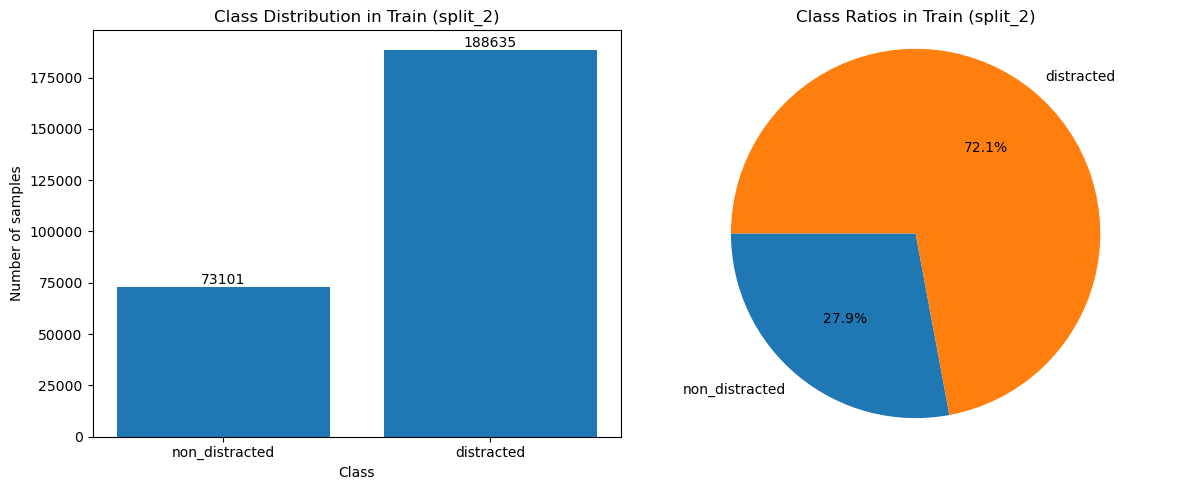
\includegraphics[width=\textwidth]{Images_Thesis/class_distribution_Kinect_color/split_2_rgb_daa/class_dist_train_sp_2_rgb_daa.png}
        \caption{Split 2: Train}
        \label{fig:Class_dist_grid_image7}
    \end{subfigure}
    \hfill
    \begin{subfigure}[b]{0.45\textwidth}
        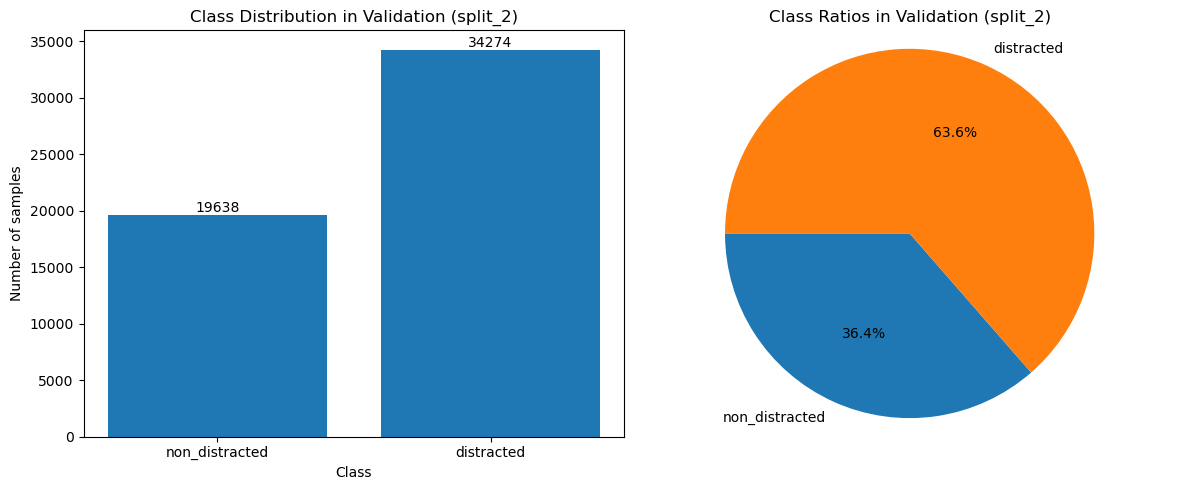
\includegraphics[width=\textwidth]{Images_Thesis/class_distribution_Kinect_color/split_2_rgb_daa/class_dist_val_sp_2_rgb_daa.png}
        \caption{Split 2: Validation}
        \label{fig:Class_dist_grid_image8}
    \end{subfigure}

    % Fifth row
    \begin{subfigure}[b]{0.45\textwidth}
        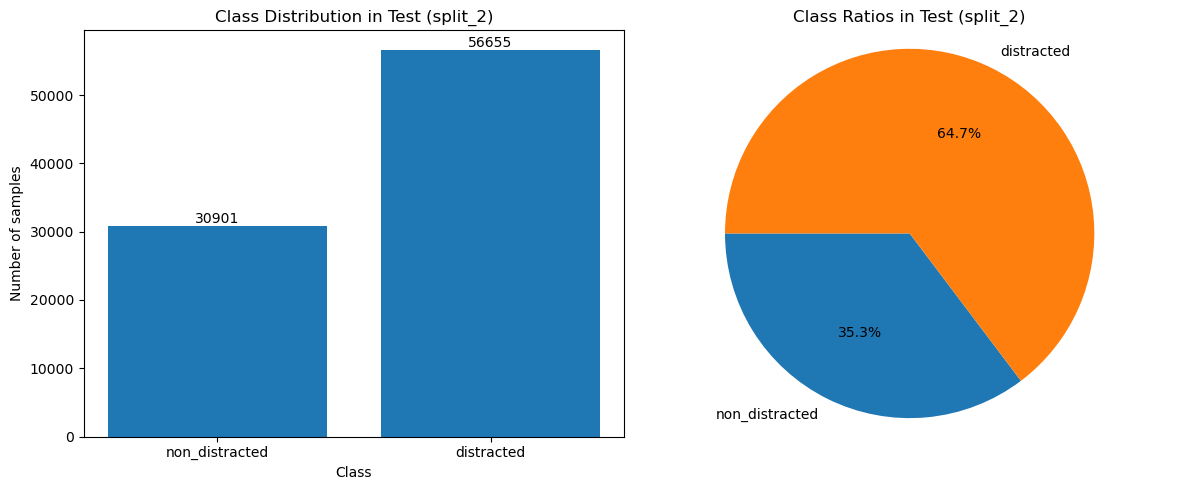
\includegraphics[width=\textwidth]{Images_Thesis/class_distribution_Kinect_color/split_2_rgb_daa/class_dist_test_sp_2_rgb_daa.png}
        \caption{Split 2: Test}
        \label{fig:Class_dist_grid_image9}
    \end{subfigure}

    \caption[Class distribution of all three splits of Kinect Color Right Top Image DAA Dataset.]{Class distribution of all three splits of Kinect Color Right Top Image DAA Dataset. In the bar plot, the x-axis corresponds to the class, while the y-axis reflects the number of images in each class. The pie chart displays the relative proportion, expressed as a percentage, of each class inside each split of the dataset. These proportions are generated based on the class ratios.}
    \label{fig:Class_dist_whole_grid_Kinect_color}
\end{figure}

\subsection{Proposed Evaluation Metrics}
As we have imbalance in the extracted image datasets, we can no longer rely on the traditional evaluation metrics like accuracy as already discussed in the chapter~\ref{chapter:related_work}. Accuracy is the ratio of correctly predicted observations to the total observations. It can be misleading in evaluating performance of a model on our imbalanced datasets. So, following the recommendations of~\citet{Survey_DL_Taghi_article, 18_wang2016training}, this thesis employs the balanced accuracy score instead of the standard accuracy score for evaluating model performance. Such metrics offer a more nuanced insight into how well models perform across all classes, irrespective of their frequency. Below is the definition and mathematical formulation of the balanced accuracy score. 

\paragraph{Balanced Accuracy:}
It is the average of the recall obtained on each class, ensuring equal treatment of each class's performance~\citep{bal_acc_paper_brodersen2010balanced, bal_acc_2_sk_learn_kelleher2015fundamentals}. 

For a binary classification problem with classes \( C_1 \) and \( C_2 \), where \( C_1 \) is considered the positive or minority class and \( C_2 \) the negative or majority class, the balanced accuracy can be mathematically expressed as follows:

Let:
\begin{itemize}
    \item \( TP \) denote the number of true positives.
    \item \( TN \) denote the number of true negatives.
    \item \( FP \) denote the number of false positives.
    \item \( FN \) denote the number of false negatives.
\end{itemize}

The recall for class \( C_1 \) (True Positive Rate) is:
\begin{equation}
\begin{aligned}
\text{Recall}_{C_1} = \frac{TP}{TP + FN}
\end{aligned}
\label{equation:4.5}
\end{equation}

The recall for class \( C_2 \) (True Negative Rate) is:
\begin{equation}
\begin{aligned}
\text{Recall}_{C_2} = \frac{TN}{TN + FP}
\end{aligned}
\label{equation:4.6}
\end{equation}

Therefore, the balanced accuracy is given by:
\begin{equation}
\begin{aligned}
\text{Balanced Accuracy} = \frac{\text{Recall}_{C_1} + \text{Recall}_{C_2}}{2}
\end{aligned}
\label{equation:4.7}
\end{equation}

With respect to this thesis, class \( C_1 \) represents the `\_non\_distracted' driver class whereas class \(C_2\) represents the `distracted' driver class. This formula ensures that both classes are equally represented in the accuracy metric, which is particularly important in cases of class imbalance~\citep{Survey_DL_Taghi_article, 18_wang2016training}.

\section{Novel Dataloader for Imbalanced Dataset}
To address the first research question of this thesis, we propose `Clustered Feature Weighting' a data loading strategy to improve imbalance in batches during model training. The methodology opted for the novel data loading is depicted in the flowchart~\ref{flowchart:flowchart_novel_dataloader_imbalanced_dataset}. This flowchart shows the step by step procedure opted for the creation of the novel dataloader titled ``ClusteredFeatureWeighting". The novel dataloader designed for this thesis aims to address the inherent bias towards the majority class in imbalanced datasets by introducing balanced batches during model training. This enhancement not only aims to mitigate model bias but also aims to improve model performance by feeding balanced batches during model training.

\subsection{Methodological Steps}
The methodology is divided into four main parts starting from model selection to final dataloader comparison as shown below. Each part of the methodology contains different design choices and verification procedures. First we will start with the explanation of the steps involved in implementing the novel dataloader, which are as follows:

\begin{enumerate}
    \item \textbf{Model Selection}: Choose a vision transformer model or encoder that has been pre-trained on the ImageNet-21K~\citep{Imagenet1k_ILSVRC15} dataset in order to obtain embeddings from the Kinect Right Top Color Drive and Act image dataset.
    
    \item \textbf{Variance Analysis}: Perform variance analysis on the collected features to assess the suitability of the selected model for feature extraction. Understanding the degree of separation between features within the same class and across different classes in the feature space is highly important. If the model is compatible with the imbalanced dataset under consideration, then move on to next step else select a suitable encoder again and verify its compatibility with the dataset under consideration by repeating the variance analysis. 
    \item \textbf{Clustering}: Arrange the features batchwise and Apply HDBSCAN~\citep{HDBSCAN_algo_campello2013density} clustering algorithm on the cosine distance between the extracted features batchwise. This step is explained in detail in the section~\ref{section:ClusteredFeatureWeighting Data Loading Strategy}.
    \item \textbf{Weight Generation}: Generate weights for a weighted random sampler based on the clustering results, to ensure diverse and representative samples in each batch.
    \item \textbf{Comparison}: Compare the effectiveness of the novel dataloader with traditional dataloader to validate improvements in batchwise imbalance. If the results are satisfactory then move on to model training or else try different weights for outliers in order to see its impact on the sampling and imbalance in batches.
\end{enumerate}

Before progressing with the methodological steps of the novel dataloader, it is essential to first establish the mathematical formulations that underpin these processes. These formulations not only guide the development and implementation of the dataloader but also serve as critical verification procedures for evaluating the efficacy of the selected model.

\begin{figure}[htbp]
\begin{center}
\tikzstyle{startstop} = [circle, 
minimum width=1cm, 
minimum height=1cm,
text centered, 
draw=black, 
fill=red!30]

\tikzstyle{io} = [trapezium, 
trapezium stretches=true, % A later addition
trapezium left angle=70, 
trapezium right angle=110, 
minimum width=3cm, 
minimum height=0.5cm, text centered, 
draw=black, fill=blue!20]

\tikzstyle{process} = [rectangle, 
minimum width=2cm, 
minimum height=0.5cm, 
text centered, 
text width=5cm, 
draw=black, 
fill=orange!20]

\tikzstyle{decision} = [diamond, 
minimum width=3cm, 
minimum height=2cm, 
text centered, 
draw=black, 
fill=green!20]
\tikzstyle{arrow} = [thick,->,>=stealth]

\begin{tikzpicture}[node distance=1.1cm]

\node (start) [startstop] {Start};
\node (in1) [io, below of=start] {Choose Encoder and do Feature Extraction};
\node (pro1) [process, below of=in1] {Perform Variance Analysis};
\node (dec1) [decision, below of=pro1, yshift=-1.5cm] {Model Compatibility};
\node (pro2a) [process, below of=dec1, yshift=-1.8cm] {Perform Clustering};
\node (pro2b) [process, right of=dec1, xshift=4.0cm] {Use Another Suitable Encoder};
\node (out1) [io, below of=pro2a] {Generate Weights};
\node (out2) [io, below of=out1] {Dataloader Comparison};
\node (dec2) [decision, below of=out2, yshift=-1.5cm] {Balanced Batches};
\node (pro3a) [process, below of=dec2, yshift=-1.5cm] {Model Training};
\node (pro3b) [process, right of=dec2, xshift=4.0cm] {Try different weights for Outliers};
\node (stop) [startstop, below of=pro3a] {Stop};

\draw [arrow] (start) -- (in1);
\draw [arrow] (in1) -- (pro1);
\draw [arrow] (pro1) -- (dec1);
\draw [arrow] (dec1) -- node[anchor=east] {Yes} (pro2a);
\draw [arrow] (dec1) -- node[anchor=south] {No} (pro2b);
\draw [arrow] (pro2b) |- (pro1);
\draw [arrow] (pro2a) -- (out1);
\draw [arrow] (out1) -- (out2);
\draw [arrow] (out2) -- (dec2);
\draw [arrow] (dec2) -- node[anchor=east] {Yes} (pro3a);
\draw [arrow] (dec2) -- node[anchor=south] {No} (pro3b);
\draw [arrow] (pro3b) |- (pro2a);
\draw [arrow] (pro3a) -- (stop);

\end{tikzpicture}
\end{center}
\caption{Methodology for Novel Dataloader for Imbalanced Dataset.}
\label{flowchart:flowchart_novel_dataloader_imbalanced_dataset}
\end{figure}

\paragraph{Mathematical Definitions and Formulations:}
To quantitatively analyze the features extracted by a model, several mathematical measures are employed. These measures are pivotal for evaluating how well a model can capture and differentiate features within and between different classes, which directly impacts the effectiveness of classification algorithms and in our case the novel dataloading startegy.

\paragraph{Intra-class Variance} (\(\sigma_{intra}^2\)):
Intra-class variance quantifies the variability or spread of feature vectors within a single class. It measures how much the features of individual samples deviate from the mean feature vector of their respective class. A lower intra-class variance indicates a high degree of similarity among the samples within the class, suggesting that the model is consistent in capturing features for a specific class~\citep{intra_class_var_pilarczyk2019intra}.

Mathematically,
\begin{equation}
\begin{aligned}
\sigma_{intra}^2 = \frac{1}{N} \sum_{i=1}^N (\vx_i - \mu)^2
\end{aligned}
\label{equation:4.8}
\end{equation}
where: \( \vx_i \) represents the feature vector of the \(i\)-th image in a class, \( \mu \) denotes the mean feature vector of that class, and \( N \) is the total number of samples in the class~\citep{intra_class_var_pilarczyk2019intra}.

\paragraph{Calculation of Class Centers:}
To calculate the class centers in a feature space extracted using a pretrained Vision Transformer model, the mean feature vector (center) for each class is computed by averaging the feature vectors of all samples within each class~\citep{intra_class_var_pilarczyk2019intra}. As there are two classes (A) `non\_distracted' and (B) distracted in the dataset under consideration, we can calculate the class centers for each class in the feature space as follows: 
If $\displaystyle N$ is the total number of sample in each class, then,

For class A:
\begin{equation}
\begin{aligned}
\text{center}_A = \text{Mean Feature Vector}_A = \mu_0 = \frac{1}{\displaystyle N} \sum_{i=1}^{\displaystyle N} \displaystyle \vx_i^A
\end{aligned}
\label{equation:4.9}
\end{equation}
where $\displaystyle \vx_i^A$ represents the feature vector of the $i$-th sample in class A.

For class B:
\begin{equation}
\begin{aligned}
\text{center}_B = \text{Mean Feature Vector}_B = \mu_1 = \frac{1}{\displaystyle N} \sum_{i=1}^{\displaystyle N} \displaystyle \vx_i^B
\end{aligned}
\label{equation:4.10}
\end{equation}
where $\displaystyle \vx_i^B$ represents the feature vector of the $i$-th sample in class B.

\paragraph{Inter-class Variance} (\(\sigma_{inter}^2\)):
Inter-class variance measures the differences between the mean feature vectors of different classes. This metric is crucial for determining how distinct the classes are from each other in the feature space. Higher values of inter-class variance suggest that the classes are more distinguishable, indicating that the model is effective in capturing diverse features necessary for differentiating between classes~\citep{inter_class_yu2022generalized}.
Mathematically,
\begin{equation}
\begin{aligned}
\sigma_{inter}^2 = (\mu_0 - \mu_1)^2
\end{aligned}
\label{equation:4.11}
\end{equation}
where: \( \mu_0 \) and \( \mu_1 \) are the mean feature vectors of two different classes.

\paragraph{Distance Between Class Centers:}
The distance between class centers is an additional metric used to evaluate the separability of classes within the feature space. This measure complements inter-class variance by providing a direct assessment of the spatial separation between class centers, which can be interpreted as an indicator of the model’s ability to partition the feature space effectively. Once the centers of each class are computed, the Euclidean distance~\citep{wikipedia_euclidean_distance} between these two centers can be calculated using the following formula:

\begin{equation}
\begin{aligned}
d(\text{center}_A, \text{center}_B) = \sqrt{\sum_{i=1}^{\displaystyle M} (\text{center}_A[i] - \text{center}_B[i])^2}
\end{aligned}
\label{equation:4.12}
\end{equation}

where, M is the size of the feature vector obtained after feature extraction or in other words M is the embedding size of the encoder used for feature extraction. For our case, M is 1280.

These metrics together create a strong foundation for evaluating the model's ability to accurately differentiate across classes using the information it extracts. They are essential for validating the feature extraction capabilities of the model, ensuring that it captures both the nuances within classes and the distinctions between different classes.

\paragraph{Cosine Similarity:}
Cosine similarity measures the cosine of the angle between two non-zero vectors in an inner product space. This measure is a reflection of the cosine of the angle between the two vectors and is calculated using the dot product of the vectors and the magnitudes (norms) of each vector~\citep{wikipedia_cosine_similarity}.

Given two vectors, $\displaystyle \vx$ and $\displaystyle \vy$, their cosine similarity, \text{similarity}($\displaystyle \vx$, $\displaystyle \vy$), is defined as:

\begin{equation}
\begin{aligned}
\text{similarity}(\displaystyle \vx, \displaystyle \vy) = \cos(\theta) = \frac{\displaystyle \vx \cdot \displaystyle \vy}{\|\displaystyle \vx\| \|\displaystyle \vy\|}
\end{aligned}
\label{equation:4.13}
\end{equation}

where:
\begin{itemize}
    \item \( \displaystyle \vx \cdot \displaystyle \vy \) is the dot product of vectors \( \displaystyle \vx \) and \( \displaystyle \vy \).\\
    If \( \displaystyle \vx = [x_1, x_2, \ldots, x_n] \) and \( \displaystyle \vy = [y_1, y_2, \ldots, y_n] \), then:

    \begin{equation}
    \begin{aligned}
    \displaystyle \vx \cdot \displaystyle \vy = x_1y_1 + x_2y_2 + \ldots + x_ny_n
    \end{aligned}
    \label{equation:4.14}
    \end{equation}
    
    \item \( \|\displaystyle \vx\| \) is the Euclidean norm (or magnitude) of the vector \( \displaystyle \vx \).
    The Euclidean norm of a vector \( \displaystyle \vx \) is defined as:
    \begin{equation}
    \begin{aligned}
    \|\displaystyle \vx\| = \sqrt{x_1^2 + x_2^2 + \ldots + x_n^2}
    \end{aligned}
    \label{equation:4.15}
    \end{equation}
    
\end{itemize}

\paragraph{Cosine Distance:}
Cosine distance is a measure derived from cosine similarity and is used to quantify the dissimilarity between two vectors. Thus, it ranges from 0 to 2, where 0 indicates identical vectors and 2 indicates completely opposite vectors~\citep{wikipedia_cosine_similarity}. It is defined as:

\begin{equation}
\begin{aligned}
\text{distance}(\displaystyle \vx, \displaystyle \vy) = 1 - \text{similarity}(\displaystyle \vx, \displaystyle \vy)
\end{aligned}
\label{equation:4.16}
\end{equation}

This formula essentially inverts the cosine similarity to provide a distance metric: when the cosine similarity is 1 (meaning \( \displaystyle \vx \) and \( \displaystyle \vy \) are identical), the cosine distance is 0; conversely, when the cosine similarity is 0 (meaning \( \displaystyle \vy \) and \( \displaystyle \vy \) are orthogonal), the cosine distance is 1.
\paragraph{Practical Use in a Matrix:}
When utilizing the pretrained vision transformer encoder model, a feature matrix \( \displaystyle \mX \) is produced for one batch. This matrix has a dimension of [1024 x 1280], where each row represents a sample vector. The batch size is 1024 and the embedding size is 1280. In this scenario, the cosine similarity can be calculated for each pair of vectors. This leads to the creation of a similarity matrix in which each member (i, j) represents the cosine similarity between the i-th and j-th vectors in \(\displaystyle \mX \). The cosine distance matrix is obtained by subtracting the similarity matrix from one. This approach for computing distances and similarities is particularly valuable in high-dimensional spaces, where the traditional Euclidean distance may lose its significance due to the curse of dimensionality. This thesis employs this approach to compute the cosine distance matrix for the HDBSCAN clustering algorithm.

Next, we will delve into the implementation details of the novel dataloader. The following section presents the pseudocode for the `Clustered Feature Weighting' data loading strategy and thoroughly explains the corresponding algorithmic workflow. This includes the strategy's implications and advantages. Following this, the section outlines the clustering process, detailing its benefits and drawbacks, and discusses its possible impact on data variability in batches and overall model training.

\subsection{ClusteredFeatureWeighting Data Loading Strategy:}
\label{section:ClusteredFeatureWeighting Data Loading Strategy}
This thesis presents a new approach to address the difficulties encountered due to imbalanced image datasets. The proposed solution is a unique data loading technique, outlined in algorithm~\ref{algorithm:Clusteredfeatureweighting} named ``ClusteredFeatureWeighting".This approach leverages advanced machine learning techniques, including clustering and weighted sampling, to enhance the training of vision models on skewed image datasets. The following section details the technical components and operational flow of this strategy, emphasizing its integration into the training process.

\begin{algorithm}
\caption{Pseudocode: ClusteredFeatureWeighting Data Loading Strategy}
\label{algorithm:Clusteredfeatureweighting}
\begin{algorithmic}[1]
\State \textbf{def} extract\_features(pretrained\_encoder, dataset):
\State \ \ \ \ features, labels, paths = [~], [~], [~]
\State \ \ \ \ \textbf{for} image, label, path \textbf{in} dataset:
\State \ \ \ \ \ \ \ \ feature = pretrained\_encoder(image)
\State \ \ \ \ \ \ \ \ features.append(feature)
\State \ \ \ \ \ \ \ \ labels.append(label)
\State \ \ \ \ \ \ \ \ paths.append(path)
\State \ \ \ \ \textbf{return} features, labels, paths

\State \textbf{def} assign\_weights(features):
\State \ \ \ \ weights = [~]
\State \ \ \ \ \textbf{for} feature\_batch \textbf{in} features:
\State \ \ \ \ \ \ \ \ cosine\_matrix = 1 - cosine\_similarity(feature\_batch)
\State \ \ \ \ \ \ \ \ clusters, outliers = HDBSCAN(cosine\_matrix)
\State \ \ \ \ \ \ \ \ \textbf{for} cluster \textbf{in} clusters:
\State \ \ \ \ \ \ \ \ \ \ \ \ weight = 1.0 / len(cluster)
\State \ \ \ \ \ \ \ \ \ \ \ \ \textbf{for} index \textbf{in} cluster:
\State \ \ \ \ \ \ \ \ \ \ \ \ \ \ \ \ weights[index] = weight
\State \ \ \ \ \ \ \ \ \textbf{for} outlier \textbf{in} outliers:
\State \ \ \ \ \ \ \ \ \ \ \ \ weights[outlier] = 0.01
\State \ \ \ \ \textbf{return} weights

\State \textbf{class} WeightedImageDataset:
\State \ \ \ \ \textbf{def} \_\_init\_\_(self, imagepath\_list, weights\_list, labels\_list):
\State \ \ \ \ \ \ \ \ self.imagepaths = [path for imagepath in imagepath\_list]
\State \ \ \ \ \ \ \ \ self.weights = [weight for weight in weights\_list]
\State \ \ \ \ \ \ \ \ self.labels = [label for label in labels\_list]
\State \ \ \ \ \textbf{def} load\_image(self, image\_path):
\State \ \ \ \ \ \ \ \ \textbf{return} Image.open(image\_path)
\State \ \ \ \ \textbf{def} \_\_getitem\_\_(self, idx):
\State \ \ \ \ \ \ \ \ image = self.load\_image(image\_path)
\State \ \ \ \ \ \ \ \ \textbf{return} image, self.imagepath, self.weights[idx], self.labels[idx]

\State \textbf{def} create\_dataloader(image\_paths, weights, labels, batch\_size):
\State \ \ \ \ dataset = WeightedImageDataset(image\_paths, weights, labels)
\State \ \ \ \ sampler = WeightedRandomSampler(weights, len(weights), rep=True)
\State \ \ \ \ \textbf{return} DataLoader(dataset, batch\_size, sampler)

\State \textbf{def} train\_model(dataloader, epochs):
\State \ \ \ \ \textbf{for} epoch \textbf{in} range(epochs):
\State \ \ \ \ \ \ \ \ \textbf{for} images, weights, labels \textbf{in} dataloader:
\State \ \ \ \ \ \ \ \ \ \ \ \ \textit{Perform training step with images and labels}

\State model = VisionTransformerModel('ImageNet-21K')
\State dataset = LoadDataset()  % Assuming dataset is pre-loaded with images, labels, paths
\State features, labels, paths = extract\_features(model.encoder, dataset)
\State weights = assign\_weights(features)
\State dataloader = create\_dataloader(paths, weights, labels, batch\_size=1024)
\State train\_model(dataloader, 100)  % Train for 10 epochs
\end{algorithmic}
\end{algorithm}

\subsection{Algorithmic Workflow}
The data loading strategy is structured around several critical phases, each tailored to optimize the model's exposure to under-represented classes in an imbalanced dataset. The algorithm~\ref{algorithm:Clusteredfeatureweighting} operates as follows:

\begin{enumerate}
    \item \textbf{Model Initialization}:
    \begin{itemize}
        \item Initialize a pre-trained vision transformer model using the ImageNet-21K dataset~\citep{Imagenet_21K_ridnik2021imagenet}. This model serves as the foundation for feature extraction, leveraging its broad, generic feature representation capabilities gained through rigorous pre-training.
    \end{itemize}

    \item \textbf{Feature Extraction}:
    \begin{itemize}
        \item For each batch of images in the training dataset, features are extracted using the pre-trained ViT specified for feature extraction. This step converts raw image data into a high-dimensional feature space where semantic similarities and differences are more visible.
        \item Extracted features, alongside true class labels and image paths, are recorded for subsequent processing.
    \end{itemize}

    \item \textbf{Clustering and Weight Assignment}:
    \begin{itemize}
        \item Within each batch, a cosine distance matrix is computed to measure the dissimilarities between all feature embeddings.
        \item HDBSCAN~\citep{HDBSCAN_algo_campello2013density}, a robust clustering algorithm suitable for handling varying cluster densities and sizes, is applied to this distance matrix. This method effectively identifies natural clusters and outliers within the data.
        \item Weights are assigned to features based on cluster membership. Each feature within a cluster receives a weight inversely proportional to the cluster size, promoting equal representation across clusters. Outliers are assigned a minimal weight of 0.01, maintaining their presence in the dataset without dominating the training process. This outlier weight requires fine tuning and can be tuned by choosing a value between 0 to 1 where 0 being the lowest weight corresponding to 0 probability in the weighted random sampler and 1 being the highest probability in the weighted random sampler for sampling.
    \end{itemize}

    \item \textbf{Weights Aggregation}:
    \begin{itemize}
        \item Weights from all batches are aggregated and paired with their corresponding image paths. This consolidated list forms the basis for the customized sampling strategy in subsequent training iterations.
    \end{itemize}

    \item \textbf{Custom Dataset and DataLoader Configuration}:
    \begin{itemize}
        \item A custom dataset class, \texttt{WeightedImageDataset}, is defined to handle the storage and retrieval of images, weights, labels, and paths.
        \item The \texttt{getitem} method is tailored to return weighted samples, ensuring that each data retrieval aligns with the predetermined weights.
        \item A \texttt{WeightedRandomSampler} is employed with the calculated weights, set with replacement to true, allowing for repeated selection of underrepresented samples, thereby enhancing their influence on the model training.
    \end{itemize}

    \item \textbf{Training Loop}:
    \begin{itemize}
        \item The training process iterates over the dataset using a PyTorch \texttt{DataLoader} configured with the custom dataset and weighted random sampler. This setup ensures that each batch is reflective of the weighted sampling strategy, focusing model training on a balanced representation of the dataset.
    \end{itemize}
\end{enumerate}

\subsection{Clustering Procedure}
We utilized HDBSCAN~\citep{HDBSCAN_algo_campello2013density}, a density based clustering algorithm known for its effectiveness in identifying clusters without predefining the number of clusters. This method is especially well-suited for data with a high number of dimensions, such as ours. Our data consists of a feature matrix with dimensions of [1024 x 1280] per batch, with a batch size of 1024. In this matrix, each row represents a sample and each column represents a feature. Clustering was based on the cosine distance matrix derived batch wise from the dataset. This metric emphasizes the angle between feature vectors, grouping together samples that are directionally similar. Post-clustering, each sample was assigned a weight. Samples within dense clusters received higher weights to emphasize their representativeness of common data patterns, while outliers were given lower weights to decrease their selection frequency in future sampling, yet keeping them within the analytical scope.

\paragraph{Advantages of the Clustering Approach}
Using HDBSCAN offers several advantages:
\begin{itemize}
    \item \textbf{Adaptability and Effectiveness}: The algorithm excels in managing diverse data shapes and densities, crucial for our complex, high-dimensional features.
    \item \textbf{Focus on Angular Similarity}: By using cosine distances, the approach is sensitive to directional similarities, which is particularly useful in datasets where traditional measures like Euclidean distance may be less informative.
    \item \textbf{Enhanced Data Sampling}: Integrating weighted random sampling ensures that the data batches used for model training are not just random collections but are reflective of the underlying data structure, potentially improving the learning process.
\end{itemize}

\subsubsection{Limitations and Challenges}
Despite its strengths, the clustering method faces some challenges:
\begin{itemize}
    \item \textbf{Dimensional Sensitivity}: Relying solely on angular differences might overlook other important aspects of data similarity or dissimilarity.
    \item \textbf{Batch Consistency}: HDBSCAN's flexibility can sometimes lead to different clustering outcomes for different batches, which might affect the consistency of sample weights and training outcomes.
    \item \textbf{Complexity in Outlier Management}: Handling outliers by assigning them low weights reduces their impact but might neglect valuable anomalous patterns that could be essential for certain predictions.
\end{itemize}

\paragraph{Impact on Data Variability and Model Training}
The strategy of weighted random sampling, particularly with replacement, ensures a comprehensive representation of data patterns:
\begin{itemize}
    \item \textbf{Balanced Variability}: This approach maintains essential data variability, crucial for preventing model overfitting. It shows the model images with central and unusual data features.
    \item \textbf{Inclusive Sampling}: Each batch includes a mix of both highly representative samples and outliers, providing a well-rounded dataset for training and enhancing the model's ability to generalize.
\end{itemize}

\section{Methodology for DataLoader Comparison}
The versions of the \gls{daa} image datasets, exhibit imbalance across their three splits. To address this, ``Clustered Feature Weighting" strategy is proposed in this thesis. However, this approach need validation for its effectiveness in producing balanced batches and increasing model performance and generalisation. This section provides details about the comparison of two data loading strategies: a traditional dataloader and the novel dataloader using a``Clustered Feature Weighting" strategy, designed to produce more balanced training batches.

\paragraph{Data Loading Strategies:}
\begin{itemize}
    \item \textbf{Traditional DataLoader:} This loader samples data directly from the imbalanced dataset, reflecting inherent class imbalances. It is used as a baseline for comparison.
    \item \textbf{Clustered Feature Weighting DataLoader:} This approach adjusts sampling probabilities to achieve a balanced class representation within each batch, thus enhancing the model's exposure to under-represented classes during training.
\end{itemize}

\paragraph{Methodology for Comparison}
The effectiveness of each dataloader on balanced distribution inside batches is evaluated based on their ability to distribute class samples evenly across batches. Ideally, for a batch size of 1024, each class should be represented by 512 samples, given that we have a binary dataset with two classes `non distracted' and `distracted' driver. The comparison focuses on how well each dataloader approximates this ideal distribution. The Kullback-Leibler (KL) divergence~\citep{KL_div_kullback1997information} is employed to quantitatively measure the discrepancy between the ideal and the actual distributions provided by the dataloaders. Kullback-Leibler divergence is a statistical metric that estimates the extent to which one probability distribution deviates from a second, reference probability distribution~\citep{KL_div_kullback1997information}.

\paragraph{Mathematical Formulation:}
The KL divergence~\citep{KL_div_kullback1997information} from a true probability distribution \( P \) to an approximate distribution \( Q \) over discrete variables is defined as follows:
\begin{equation}
\begin{aligned}
D_{KL}(P \parallel Q) = \sum_{i} P(i) \log\left(\frac{P(i)}{Q(i)}\right)
\end{aligned}
\label{equation:4.17}
\end{equation}

where, \( P \), the uniform distribution per batch, is:

\begin{equation}
\begin{aligned}
P = \left[\frac{1}{2}, \frac{1}{2}\right]
\end{aligned}
\label{equation:4.18}
\end{equation}

and \( Q \), the observed distribution from a dataloader for each batch, is calculated as:

\begin{equation}
\begin{aligned}
Q = \left[\frac{\text{number of `non\_distracted' samples}}{1024}, \frac{\text{number of `distracted' samples}}{1024}\right]
\end{aligned}
\label{equation:4.19}
\end{equation}

\paragraph{Criteria for Comparison:}
A lower KL divergence indicates a closer approximation to the ideal distribution, signifying a more effective dataloader in terms of managing class balance~\citep{KL_div_kullback1997information}. The KL divergence values against batch numbers for both dataloaders has been plotted. This visual analysis helps identify which dataloader consistently provides a more balanced class distribution across batches.

\section{Methodology for Model Training and Evaluation}
\label{section:Methodology for Model Training and Evaluation}
This section details the methodologies used across experiments to enhance driver distraction detection through supervised and self-supervised learning-based pre-trained encoders. We explore supervised and self-supervised learning-based pre-trained encoders, grayscale augmentation, and novel data loading to assess their impact on model accuracy and generalizability. Each experiment tests the models under different conditions, focusing on their adaptability across visual modalities and camera perspectives, which is critical for real-world automotive applications. In the following chapter, we will conduct thorough experiments to gain a deeper understanding of how various methods of training encoders accurately identify drivers who are distracted.

\subsection{Experiment 1: Supervised Learning Based Encoder}
\label{section:Methodology Experiment 1: Supervised Learning Based Encoder}
We employed the Kinect Color DAA Image dataset, captured from a right-top camera view, for training and evaluation. Figure~\ref{fig:method_flow_chart_d_a_without_aug} illustrates the workflow for this experiment. We utilized a vision transformer encoder (vit\_b\_16)~\citep{vit_b_16_pytorch}, pre-trained on the Imagenet-1K~\citep{Imagenet1k_ILSVRC15} dataset using a supervised learning approach accessed from the torchvision library. This model, serving as a frozen backbone, extracts features for the downstream task of driver distraction detection. Our objective is to assess the effectiveness of a pre-trained encoder, using supervised learning, in identifying distracted drivers. We added a linear layer, distinguishing between distracted and non-distracted drivers, atop the encoder. This layer underwent fine-tuning on the dataset for 100 epochs, guided by hyperparameters derived from our search discussed in the subsequent chapter. Pre-trained model specific data transformations were applied during the training and evaluation phases. We employed the cross-entropy loss~\citep{cross_entropy_loss_mao2023cross} as our loss function, utilizing a batch size of 1024. We evaluated the performance of the trained model by testing it on previously unseen datasets from the Kinect Color Right Top view Image DAA test datasets.

\begin{figure}[h]
\begin{center}
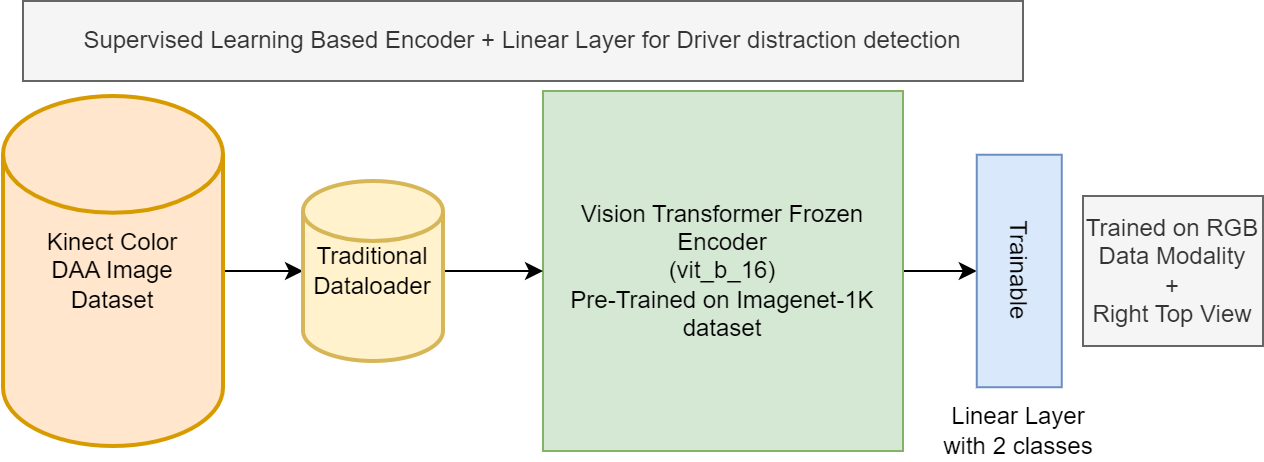
\includegraphics[width=0.8\textwidth]{Images_Thesis/methodology_images/methodology_flowchart_d_a_without_augmentation_final_2.png}
\end{center}
\caption[Methodology for supervised learning based pre-trained encoder for downstream task of driver distraction detection.]{Methodology for supervised learning based pre-trained encoder for downstream task of driver distraction detection.}
\label{fig:method_flow_chart_d_a_without_aug}
\end{figure}

\subsection{Experiment 2: Supervised Learning Based Encoder with Gray scale Augmentation}
\label{section:Methodology 2 Experiment 2: Supervised Learning Based Encoder with Gray scale Augmentation}
Figure~\ref{fig:method_flow_chart_d_a_with_aug} outlines the methodology for this experiment, which mirrors Experiment 1 with a significant variation: the addition of grayscale augmentation. This experiment was designed to explore the impact of grayscale augmentation on model generalization, particularly under low-light or night time driving conditions where color images may offer limited information. We hypothesized that grayscale images might yield better generalizability in such scenarios. Thus, we trained our hybrid classifier with grayscale augmentation for 100 epochs and subsequently evaluated its effectiveness.
\begin{figure}[h]
\begin{center}
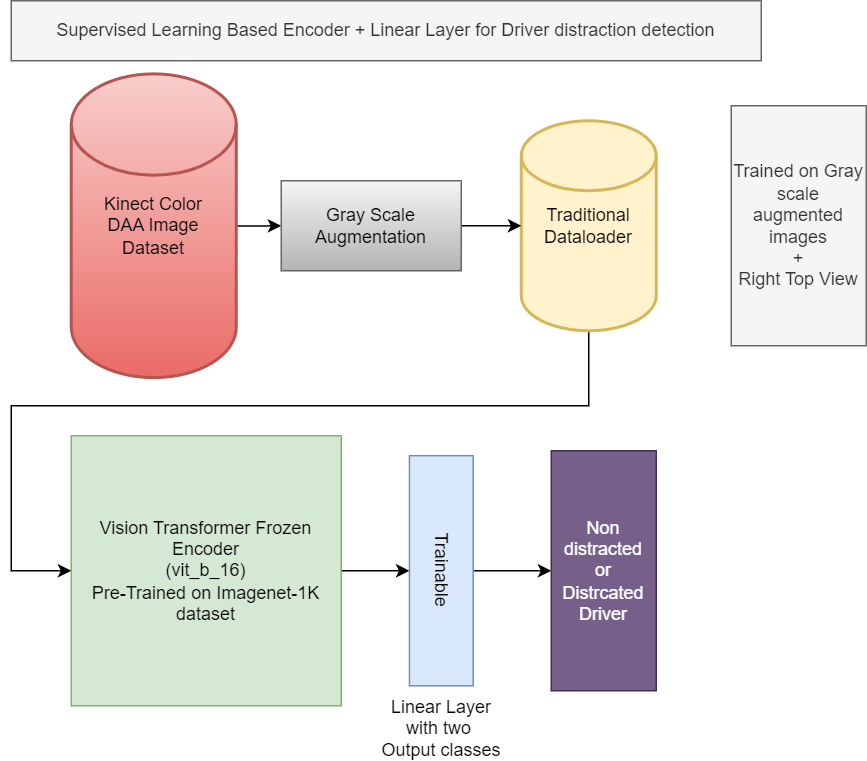
\includegraphics[width=0.8\textwidth]{Images_Thesis/methodology_images/methodology_flowchart_d_a_with_augmentation.png}
\end{center}
\caption[Methodology for supervised learning based pre-trained encoder with gray scale augmentation for downstream task of driver distraction detection.]{Methodology for supervised learning using a pre-trained encoder with grayscale augmentation for driver distraction detection. The figure shows grayscale transformations applied during data loading, incorporating IR modality knowledge to fine-tune a linear layer on a frozen encoder.}
\label{fig:method_flow_chart_d_a_with_aug}
\end{figure}

\subsection{Experiment 3: Self-Supervised Learning (SSL) Based Encoder}
\label{section:Methodology Experiment 3: Self-Supervised Learning Based Encoder}
The methodology for this experiment is depicted in figure~\ref{fig:method_flow_chart_d_a_ssl}. We utilized a vision transformer encoder, vit\_b\_14~\citep{dinov2_github}, trained with the DINOv2 SSL method on the extensive, unlabeled LVD-142M~\citep{dinov2_oquab2023dinov2} dataset. The encoder, frozen to preserve its feature-extracting capabilities, processes image batches to serve as inputs to a linear classifier designed for detecting driver distractions. This setup allowed us to train the linear layer of the model on the color modality with a right top view and evaluate its performance on unseen test datasets. This experiment aims to compare the performance of linear layer fine tuned on top of self-supervised learning-based frozen encoder against Experiments 1 and 2. For a balanced comparison, we will evaluate the 100th checkpoint of the finely-tuned linear layers across all experiments, assessing both validation and test balanced accuracy scores.

\begin{figure}[h]
\begin{center}
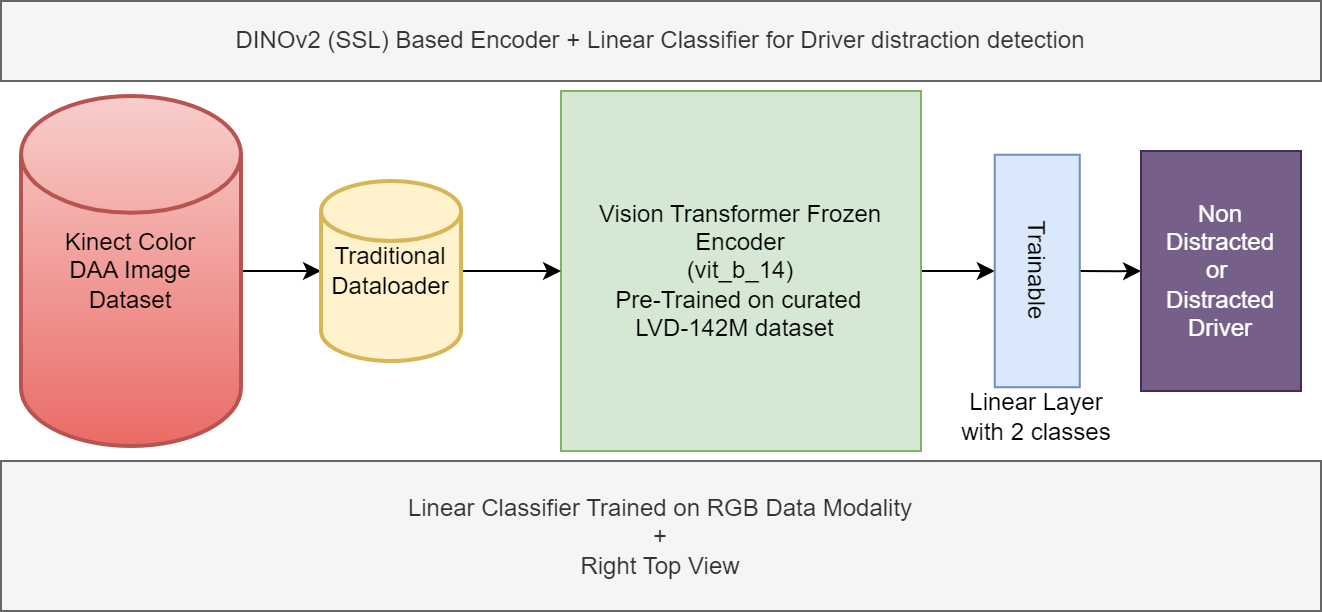
\includegraphics[width=0.8\textwidth]{Images_Thesis/methodology_images/methodology_flowchart_ssl_d_a.png}
\end{center}
\caption[Methodology for self-supervised learning based pre-trained encoder for downstream task of driver distraction detection.]{Methodology for self-supervised learning based pre-trained encoder (DINOv2 vit\_b\_14) for downstream task of driver distraction detection. The figure depicts the traditional dataloading of the Kinect Color DAA dataset and fine-tuning of a linear layer on top of frozen encoder for downstream driver distraction detection task.}
\label{fig:method_flow_chart_d_a_ssl}
\end{figure}

\subsubsection{Choice of Linear Evaluation protocol}
The authors of the~\citep{dinov2_oquab2023dinov2} have used both kNN and linear evaluation protocols in their research. But in this thesis, the DINOv2 based `vit\_b\_14' encoder~\citep{dinov2_oquab2023dinov2}, pretrained on curated LVD-142M unlabeled dataset, is tested using the linear probing on the Kinect color right top drive and act image dataset. This decision is guided by several factors:
\begin{itemize}
    \item \textbf{Computational Efficiency:} Linear evaluation requires considerably less computational resources compared to full fine-tuning and can be executed relatively quickly~\citep{ssl_codebook_balestriero2023cookbook}.
    \item \textbf{Direct Assessment of Representational Quality:} Since linear probing focuses purely on the discriminative power of the pre-trained features without allowing significant model adaptation, it provides a clear indication of the quality of the \gls{ssl}-induced features~\citep{ssl_zhang_2016_colorful, ssl_codebook_balestriero2023cookbook}.
    \item \textbf{Practical Relevance:} Training a linear classifier on a fixed backbone roughly replicates real-world scenarios, where \gls{ssl} models are often used as feature extractors in larger systems~\citep{ssl_zhang_2017split, ssl_codebook_balestriero2023cookbook}.
\end{itemize}

\subsection{Experiment 4: SSL Based Encoder with Clustered Feature Weighting}
\label{section: Methodology Experiment 4: Self-Supervised Learning Based Encoder with Clustered Feature Weighting Data-loading}
Figure~\ref{fig:method_flow_chart_d_b_ssl} details this experiment's methodology, highlighting the use of a clustered feature weighting data loading technique, a deviation from traditional data loading approaches. This method is expected to enhance model training and generalization across unseen datasets and different modalities or views. The same encoder and linear layer configuration from Experiment 3 is employed, but with the clustered feature weighting strategy during model training.
\begin{figure}[h]
\begin{center}
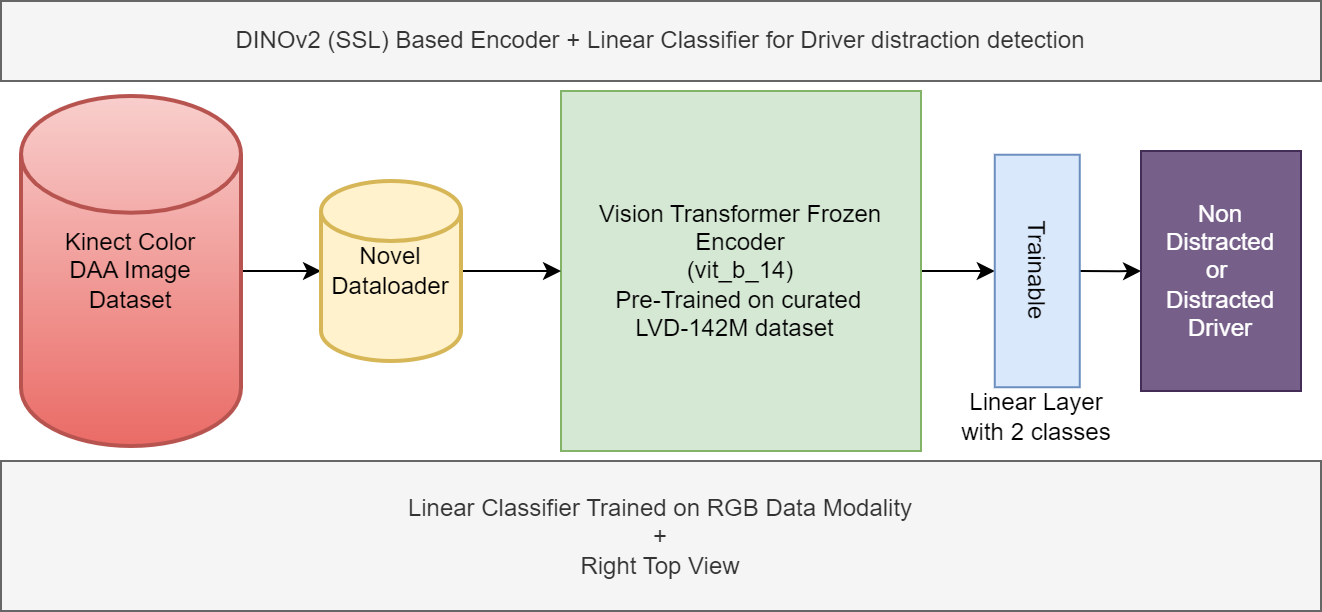
\includegraphics[width=0.8\textwidth]{Images_Thesis/methodology_images/methodology_flowchart_d_b_ssl.png}
\end{center}
\caption[Methodology for self-supervised learning based pre-trained encoder with Clustered Feature Weighting Data-loading for downstream task of driver distraction detection.]{Methodology for self-supervised learning based pre-trained encoder (DINOv2 vit\_b\_14) with Clustered Feature Weighting Data-loading for downstream task of driver distraction detection. In the figure novel dataloader corresponds to Clustered Feature Weighting based dataloader.}
\label{fig:method_flow_chart_d_b_ssl}
\end{figure}

\paragraph{Data Transformations in Experiment 3 and 4:}
Data transformation strategies are crucial for training robust models. We employed the same data transformation strategy for both training and evaluation phases as described and used in~\citep{dinov2_oquab2023dinov2} for linear probing.
\paragraph{Training Transforms:}
The training transforms includes a series of transformations to simulate diverse viewing conditions:
\begin{itemize}
    \item \textbf{RandomResizedCrop}: Applied with bicubic interpolation to preserve image quality while adjusting sizes. The crop size used is 224.
    \item \textbf{RandomHorizontalFlip}: Conditionally applied based on a 0.5 probability to introduce horizontal asymmetry.
    \item \textbf{MaybeToTensor}: Ensured all inputs were converted to tensors to accommodate different formats.
    \item \textbf{Normalization}: Used predefined ImageNet~\citep{Imagenet1k_ILSVRC15} mean and standard deviation values to standardize inputs.
\end{itemize}

\paragraph{Evaluation Transforms:}
The evaluation transforms aimed for consistency and reproducibility:
\begin{itemize}
    \item \textbf{Resize and CenterCrop}: First the image is resized to a size 256 using bicubic interpolation to ensure high-quality image representation at standard dimensions. Then the CenterCrop with crop size 224 is applied.
    \item \textbf{MaybeToTensor and Normalization}: Consistently prepared and standardized inputs, similar to training transforms.
\end{itemize}

\subsection{Methodology for Cross-Modality Generalization Evaluation}
\label{section:Methodology for Cross-Modality Generalization Evaluation}
Figure~\ref{fig:method_flow_chart_cross_modality_gen} illustrates the cross-modality generalization approach. We evaluated the 100th epoch checkpoints of the trained encoders on the KIR Right Top and NIR Front Top IR datasets, which present different imaging modalities (IR) compared to the color data used in model training. This experiment seeks to understand the adaptability of models to different sensory information, relevant in diverse lighting conditions.

\begin{figure}[h]
\begin{center}
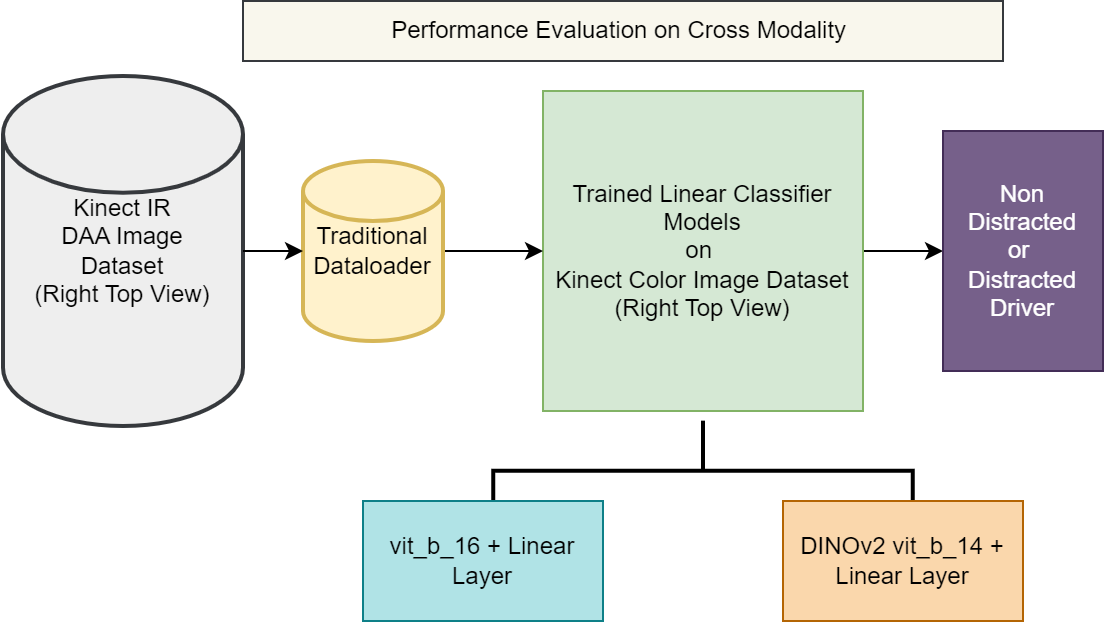
\includegraphics[width=0.8\textwidth]{Images_Thesis/methodology_images/methodology_cross_modality_generalisation.png}
\end{center}
\caption[Methodology for cross-modality generalisation.]{Methodology for cross-modality generalisation for downstream task of driver distraction detection. KIR Right Top view dataset only differs in the modality of data when compared with Kinect Color Right Top view dataset. Hence, using Kinect IR DAA test sets, the cross-modality evaluation across all four experimental scenarios is performed.}
\label{fig:method_flow_chart_cross_modality_gen}
\end{figure}

\subsection{Methodology for Cross-View Generalization Evaluation}
\label{section:Methodology for Cross-View Generalization Evaluation}
Figure~\ref{fig:method_flow_chart_cross_view_gen} shows the methodology for cross-view generalization. Here, we assess the models trained on the right view Kinect color image DAA dataset against the NIR Front Top dataset, which provides a different camera perspective. This experiment aims to verify the models' robustness to varying viewpoints, simulating real-world scenarios where camera angles can differ unexpectedly.

\begin{figure}[h]
\begin{center}
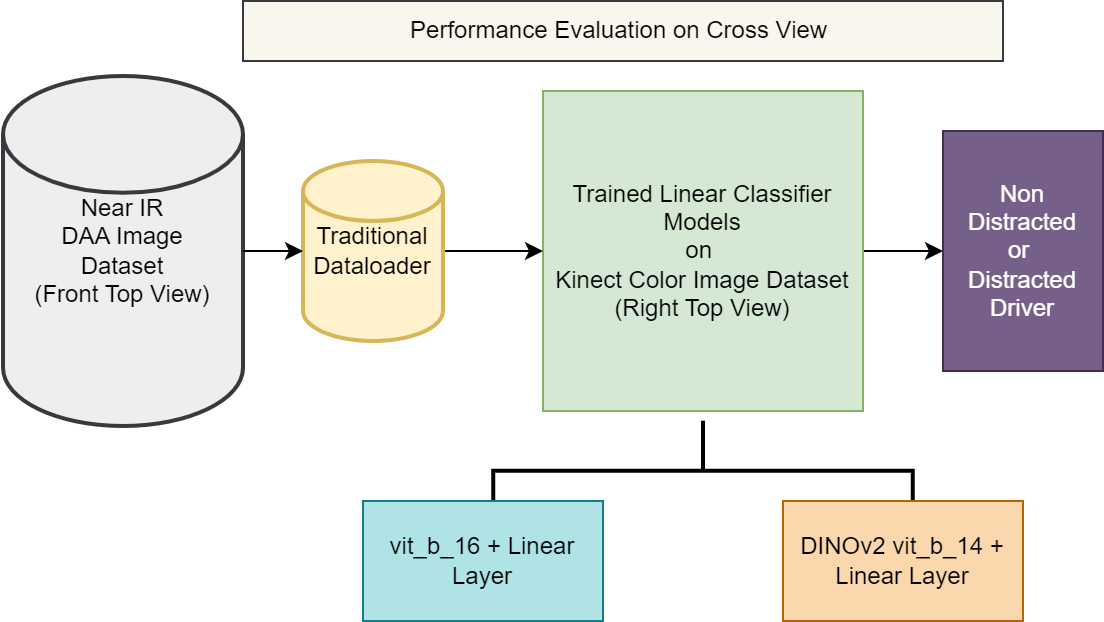
\includegraphics[width=0.8\textwidth]{Images_Thesis/methodology_images/methodology_cross_view_generalisation.png}
\end{center}
\caption[Methodology for cross-view generalisation.]{Methodology for cross-view generalisation for downstream task of driver distraction detection. In the figure, the NIR DAA dataset is used with front top view and Ir modality for cross-view and cross modality generalisation. This evaluation done in all four experiments using both types of encoder under consideration as depicted in the figure.}
\label{fig:method_flow_chart_cross_view_gen}
\end{figure}


